\documentclass{article}
\usepackage[utf8]{inputenc}
\usepackage{imakeidx}

\usepackage{natbib}
\usepackage{graphicx}
\usepackage{listings}   
\usepackage{tcolorbox}
% Include the listings-package
\lstset{breaklines}

\begin{document}

\begin{titlepage}

    \begin{center}
        \vspace*{1cm}
        \Huge
        \textbf{M-N-K Game}
            
        \vspace{0.5cm}
        \LARGE
         Relazione del progetto per l'insegnamento di Algoritmi e Strutture Dati \\
        
            
        \vspace{1.0cm}
        \vfill
        Erik Koci M. 0000997662 \\ 
        Paolo Ceroni M. 0000978232\\
        \vspace{0.8cm}
            
        
            
        \Large
        Dipartimento di Informatica\\
        Università di Bologna\\
        A.A 2020/2021\\
            
    \end{center}
\end{titlepage}


\tableofcontents
\newpage

\section{Problema}
\begin{itemize}
    \item Sviluppare un giocatore software in grado di giocare in modo ottimale a tutte le istanze possibili del (M,N,K)-game.
    \item Il numero di mosse intelligenti cresce esponenzialmente rispetto alla dimensione della matrice di gioco ed il numero di simboli da allineare.
    \item Tramite una dimostrazione per furto di strategia si può dimostrare che il secondo giocatore non può avere una strategia che gli assicuri la vittoria.
\end{itemize}

\begin{figure}[h!]
\centering
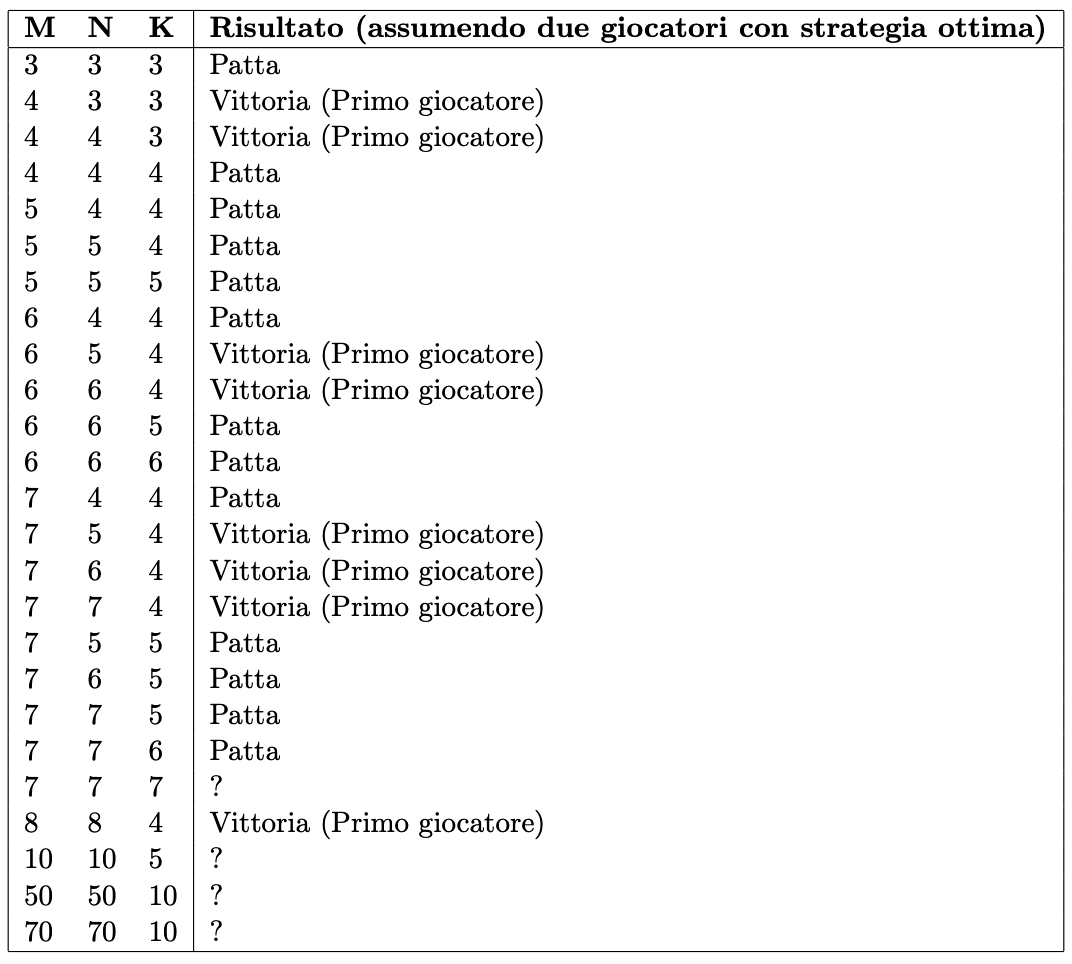
\includegraphics[width=8cm,height=8cm]{img/match.png}
\caption{Esempi di configurazione m,n,k}
\label{fig:universe}
\end{figure}

\section{Scelte progettuali}
    Nello sviluppo progettuale del metodo \textbf{selectCell()} inizialmente abbiamo optato per un algoritmo di ricerca \textbf{negamax}, il quale è una variante dell'algoritmo  \textit{minmax}.\\
    Questa tipologia di algoritmo viene spesso utilizzata nei giochi a turni tra due o più giocatori basandosi sulla somma di punteggi di ogni mossa. Successivamente le valutazioni effettuate dall'algoritmo saranno salvate in una matrice la quale ci permetterà di avere una \textbf{cache} interna di gioco, nella quale potremmo accedere nel caso trovassimo una combinazione valutata. Questo tipo di implementazione si basa sulla \textbf{programmazione dinamica}.
    
    \subsection{Negamax}
    L'algoritmo \textbf{negamax} \cite{Negamax} si basa sul fatto che $max(a.b) = -min(-a,-b)$ più precisamente, il valore di una posizione per il giocatore \textit{A} in questa tipologia di gioco è la negazione del valore per il giocatore \textit{B}.\\
    Pertanto, il giocatore cercherà una mossa che massimizzi la negazione del valore risultante della mossa. Quest'ultima deve essere stata valutata per definizione dall'avversario.\\
   Il ragionamento applicato funziona indipendentemente dal fatto che \textit{A} o \textit{B} faccia una mossa. Ciò implicà che è possibile utilizzare un'\textbf{unica procedura} per valutare entrambe le posizioni.\\
   \textit{Negamax} è una semplificazione più elegante dell'algoritmo \textbf{minmax} che richiede che \textit{A} selezioni la mossa con il valore di massimo mentre \textit{B} seleziona la mossa con il valore di minimo.\\
    Una volta terminata una esecuzione di gioco, la funzione \textit{evaluate} determinerà il punteggio da attribuire a seconda del \textit{game state}.
   
    \begin{figure}[h!]
    \centering
    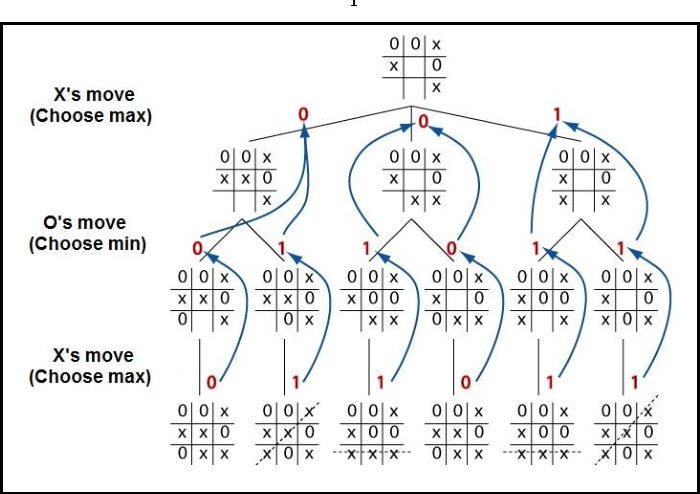
\includegraphics[width=10cm,height=6cm]{img/test.png}
    \caption{Negamax}
    \label{fig:universe}
    \end{figure}
   \subsubsection{Pseudocodice Negamax} 
    \lstset{language=java, numbers=left,numbersep=8pt,  }
    \begin{lstlisting}[frame=single]  
 function negamax(node, depth, color) is
    if depth = 0 nodo terminale  then
      return color * valore euristico
    value := -infinity
    for each child of node do
      value := max(value,-negamax(child, depth-1,-color)) 
    return value
    \end{lstlisting}
    
    
    
    
    \subsection{Zobrist Hashing}
    Prima di parlare della \textit{tabella di trasposizione} è necessario capire la funzione di hashing utilizzata.
    L'\textbf{hashing di Zobrist} \cite{zobrist} inizia generando casualmente interi di tipo \textit{long}, per ogni possibile elemento posizionabile nella nostra tabella di trasposizione. In seguito, ogni volta che una cella verrà \textit{marcata} o \textit{demarcata} andremo a \textit{ricalcolare} il valore di hashing effettuando una operazione di \textbf{xor} tra la cella marcata della \textit{board} e il valore di \textit{hashing random} generato precedentemente. 
    
    \subsubsection{Pseudocodice Zobrist Hashing}
    \lstset{language=java, numbers=left,numbersep=8pt,  }
    \begin{lstlisting}[frame=single]  
function init_zobrist():
    # riempimento con numeri random
    table := a 2-d array  
    for each cell on the board :
        table[i][j] := random_long()

function findhash(board):
    hash = 0
    for each cell on the board :
        if cell is not empty :
            piece = board[cell]
            # esegue lo xor
            hash ^= table[cell][piece]
    return hash
    \end{lstlisting}
    
    \subsection{Tabella di trasposizione}
    La tabella di trasposizione \cite{Transposition_Table} è un \textbf{database} che memorizza i risultati delle ricerche eseguite in precedenza. È un modo per ridurre notevolmente lo spazio di ricerca di un albero di gioco con scarso impatto negativo.\\
    Normalmente gli algoritmi risolutivi per i giochi finiti, come nel nostro caso, utilizzano metodi di \textbf{forza-bruta}, dove vengono analizzate tutte le possibili mosse durante la loro ricerca.\\
    In questo modo vengono incontrate più e più volte le stesse posizioni, ma da sequenze di mosse differenti. Le tabelle di trasposizione quindi, \textbf{limitano} queste inutili \textbf{iterazioni}.\\
    Per salvare i valori all'interno della tabella è necessario utilizzare una funzione di \textbf{hashing}.
    Le funzioni \textit{hash} convertono le posizioni in un numero scalare quasi unico, consentendo un rapido calcolo dell'indice e una verifica delle posizioni memorizzate.\\\\\\\\
    Esistono diverse tecniche di hashing le più diffuse sono:
    \begin{itemize}
        \item Zobrist Hashing
        \item BCH Hashing
    \end{itemize}   
    Nel nostro algoritmo è stato utilizzando l'hashing di \textbf{Zobrist} aggiornando in modo incrementale il valore durante la creazione e l'annullamento della mossa. Una volta calcolato il valore di hashing andremo a inserire nella tabella di trasposizione i seguenti dati da memorizzare:
    \begin{enumerate}
        \item Profondità di ricerca
        \item Migliore mossa trovata
        \item Valore della migliore mossa trovata
        \item Tipo di valore trovato
    \end{enumerate}
    
    \subsection{Iterative Deepening}
    Un notevole miglioramento che permette la scelta di una mossa migliore è dato dall'\textit{iterative deeepening} \cite{Iterative_Deepening}, il quale inizia con una ricerca in un solo strato, e successivamente \textbf{incrementa} la \textbf{profondità} di ricerca ed esegue un'altra ricerca.\\ Questo processo viene ripetuto fino all'esaurimento del \textbf{tempo} assegnato.\\ In caso di \textit{ricerca incompleta}, avremo sempre la possibilità di ripiegare sulla mossa selezionata nell'ultima iterazione della ricerca. \\
    Ogni qualvolta una nuova mossa verrà trovata, essa andrà a \textbf{sovrascrivere} la precedente ormai diventata superflua.\\
    In questo modo possono essere accettati anche i risultati delle \textbf{ricerche parziali}, anche se, in caso di un forte calo del punteggio euristico ottenuto è opportuno dedicare un po' di tempo in più, poiché la prima alternativa è spesso una cattiva mossa.
    
    
    
        \subsubsection{Pseudocodice Iterative Deepening}
    \lstset{language=java, numbers=left,numbersep=8pt,  }
    \begin{lstlisting}[frame=single]  
function IterativeDeepening(root, goal){ #profondita max
  for(profondita = 1; root!=goal; profondita++):
    root = DLS(root,goal,profondita) 
}

function DLS(nodo, goal, profondita){
  if(profondita >= 0):
    if(nodo == goal): return nodo
    foreach(child in visita(nodo)):
        DLS(child, goal, profondita-1)
}
    \end{lstlisting}
    


    \subsection{Valutazione euristica}
    Una funzione \textit{euristica} permette di determinare il \textbf{valore} di una tabella a seconda della possibilità di vittoria. L'implementazione di una valutazione euristica è indispensabile per permettere il giusto funzionamento dell'algoritmo \textbf{Negamax}.\\
    A livello pratico, non conoscendo il valore esatto delle tabelle, cerchiamo di fare un'approssimazione in modo tale che venga scelta la tabella con \textit{maggiore} probabilità di vittoria.\\
    Nella nostra implementazione valutiamo ogni riga, colonna, diagonale e antidiagonale passante per l'ultima cella marcata, ma fermandoci a distanza \textbf{K} (o ai limite della tabella) in ogni direzione. Per cui ogni sequenza che andiamo a valutare avrà una lunghezza minore o uguale a \textbf{2K+1}.\\ Per ciascuna sequenza si valutano le sottosequenze \textbf{aperte} e \textbf{semiaperte} dei rispettivi giocatori, dando peso in particolari alle sequenze di lunghezza $K-1$, $K-2$ e $K-3$, assegnando un \textit{punteggio} stabilito dalla funzione \textit{seriesBonus}.\\
 
 
     \subsubsection{Pseudocodice heuristic:}
    \lstset{language=java}
    \begin{lstlisting}[frame=single]  
function heuristic() {
  if(B.getMarkedCells().length > 0) {
      MNKCell c = lastMarkedCell();
      int res = 0,i,j;
      //row evaluation
      i = c.i;
      j = c.j - leftSide;
      res += depthCell(i,j,0,1,leftSide+rightSide+1);
      
      //column evaluation
      i = c.i - aboveSide;
      j = c.j;
      res += depthCell(i,j,1,0,aboveSide+belowSide+1);
      
      //diagonal evaluation
      i = c.i - leftUpSide;
      j = c.j - leftUpSide;
      res += depthCell(i,j,1,1,leftUpSide+rightDownSide+1);
      
      //antidiagonal evaluation
      i = c.i - rightUpSide;
      j = c.j + rightUpSide;
      res += depthCell(i,j,1,1-1, rightUpSide+leftDownSide+1);
}
    \end{lstlisting}
    \newpage
    \subsubsection{Pseudocodice depthCell:}
   \lstset{language=java}
    \begin{lstlisting}[frame=single]   
function depthCell(i,j, direction ,len) {
  for(z=0;z<len;z++):
    if(B.cellState(i+z*direction.i,j+z*directon.j) = P1):
      value = value + seriesBonus(c1series, maxSeries, marked);
    endif
    if(B.cellState(i+z*dir_i,j+z*dir_j) = P2):
      value = value - seriesBonus(c2series, maxSeries, marked);
    endif
  endfor
}
    \end{lstlisting}
    
    \subsubsection{Pseudocodice seriesBonus:}
    \lstset{language=java}  
    \begin{lstlisting}[frame=single]
function seriesBonus(n,consecutive,marked) {
  res := 0
  if n greater then K:
    if consecutive greater then K-3:
      if consecutive greater then K-1:
        res := res + 5_000_000;
      endif
      else if consecutive greater then K-2:
        res := res + 500_000;
      endif
      else if consecutive >= K-3
        res := res + 10_000
      endif
    endif
    else
      if marked greater then K-1:
        res := res + ((marked)/(n-marked))*100_000;
      endif
  endif
  return res;
}

    \end{lstlisting}
 
 
 
 
 
    
    
  
\newpage
    \subsubsection{Pseudocodice markMyWinningCell:}
    \lstset{language=java}
    \begin{lstlisting}[frame=single]  
function markMyWinningCell(MNKBoard B) {
  for each freeCell do
    if(markCell(i,j) == myWin) 
       return cell
}
    \end{lstlisting}
    \subsubsection{Pseudocodice markEnemyWinningCell:}
    \lstset{language=java}
    \begin{lstlisting}[frame=single]  
function markEnemyWinningCell(MNKBoard B) {
    markCell(i,j)
    for each freeCell do
      if(markCell(i,j) == yourWin) 
         B.unmarkCell()
         B.unmarkCell()	       
         B.markCell(i,j)   
         return cell(i,j)
      else 
         B.unmarkCell()       
}
    \end{lstlisting}

        
    
 %----------------------------------------------------------------------

     \subsection{Possibili euristiche precedentemente applicate}
    A livello di strategie di implementazione, oltre all'\textbf{euristica} citata precedentemente, sono state implementate anche altri metodi con scarsi risultati:
    
    \begin{enumerate}
        \item Ricavare e analizzare solo le celle vicine a \textbf{distanza} minore-uguale a \textbf{K}. 
    \subsubsection{Pseudocodice $\leq$ K}
    \lstset{language=java}
    \begin{lstlisting}[frame=single]  
function removeBadMoves(MNKBoard B) {
    for each markedCell do
        for each k-distance Free-cell do 
            if(i+k < B.M) add(i+k,j)
    	    if(j+k < B.N) add(i,j+k)
    	    if(i-k >= 0) add(i-k,j)
    	    if(j-k >= 0) add(i,j-k)
    	    if(i+k < B.M and j+k < B.N) add(i+k,j+k)
    	    if(i+k < B.M and  j-k >= 0) add(i+k,j-k)
    	    if(i-k >= 0 and j+k < B.N) add(i-k,j+k)
    	    if(i-k >= 0 and j-k >= 0) add(i-k,j-k)
    return possibleValue;
}
    \end{lstlisting}
        
        \item scegliere una mossa \textbf{vicina} a una cella avversaria nel caso in cui non si riesca a ricavare una mossa "vincente". (in questo modo con configurazioni m,n,k di grandi dimensione abbiamo più \textbf{probabilità} di selezionare una cella vincente. 
        
    \subsubsection{Pseudocodice nearCell}
    \lstset{language=java}
    \begin{lstlisting}[frame=single]  
function getBestMoves(MNKBoard B) {
    for each freeCell do
        if (cellState(i+1,j) != FREE) add(i,j);
        if (cellState(i,j+1) != FREE) add(i,j);
	if (cellState(i-1,j) != FREE) add(i,j);
        if (cellState(i+1,j+1) != FREE) add(i,j);
	if (cellState(i+1,j-1) != FREE) add(i,j);
	if (cellState(i-1,j+1) != FREE) add(i,j);
	if (cellState(i-1,j-1) != FREE) add(i,j);
	if (cellState(i,j-1) != FREE) add(i,j);
    return singolCellUseful;
}
    \end{lstlisting}
        
 
    \end{enumerate}
    
    
    
    \section{Conclusioni}
    La funzione \textit{seriesBonus} usata per l'euristica richiederebbe dei valori particolari per rispecchiare in modo ottimale il valore della tabella. Dopo diversi tentativi abbiamo trovato dei valori che restituiscono un valore soddisfacente.\\
    Dal punto di vista computazionale è stata data una stima approssimativa dovuta alla tipologia di algoritmo, poiché non è possibile definire un numero massimo di nodi visitati.\\
    In conclusione gli algoritmi applicati hanno dato un riscontro sufficientemente positivo sull'efficacia del player implementato.
    
    \subsection{Complessità computazionale}
    La complessità computazionale del metodo \textit{selectCell()} deriva maggiormente dall'algoritmo \textit{Negamax} e \textit{Iterative Deepening}.\\
    \textit{Negamax} ha costo computazionale pari a $O(m^d)$
    dove $m$ sono le mosse per giocatore e $d$ indica la profondità della mossa; tuttavia se l'ordinamento è perfetto il numero di posizioni ricercate diventa $O(\sqrt{m^d})$.\\
    \textit{Iterative Deepening} ha un costo trascurabile di $O(d)$ dove $d$ indica la profondità della soluzione più vicina alla radice.\\
    Invece, la tabella di trasposizione implementata assieme alla funzione di hashing di Zobriest ha un costo costante $O(1)$.\\
    Un altro fattore importante da osservare è l'euristica che ha costo computazionale pari a $O((2K+1)\times 4)=O(K)$ dove $K$ è il numero di celle da allineare.


\subsection{Alternative strategie progettuali}
Possibili miglioramenti/strategie applicabili possono migliorare ulteriormente l'efficacia di gioco del nostro giocatore. Metodi e strategie potrebbero essere:
\begin{itemize}
    \item L'uso di una migliore euristica di gioco, come ad esempio le seguenti \cite{cari}:
    \begin{itemize}
        \item Euristica di \textbf{ABDOULAYE}  dove viene implementato è gestito il concetto di \textbf{threat}.
        \item Euristica di \textbf{Shevchenko}, dove vengono analizzate le celle presenti per righe, colonne e diagonali
        \item Euristica di \textbf{Chua Hock Chuan}, in cui ci basiamo sugli allineamenti di entrambi i giocatori in tutte le direzioni.
    \end{itemize}
    \item Adottare il metodo di \textbf{Monte Carlo} \cite{Monte_Carlo_method}, dove andiamo a campionare casualmente delle combinazioni di tabelle per ottenere dei risultati numerici
    \item La \textbf{Ricerca quiescenza} \cite{Quiescence_search} dove una volta effettuata la valutazione delle mosse, essa viene rinviare senza considerare le mosse future della posizione, fino a quando non è sufficientemente stabile per essere valutata. 
\end{itemize}

\begin{thebibliography}{9}

\bibitem{Negamax}
https://en.wikipedia.org/wiki/Negamax

\bibitem{zobrist}
    https://www.geeksforgeeks.org/minimax-algorithm-in-game-theory-set-5-zobrist-hashing/

\bibitem{Transposition_Table}
    https://www.chessprogramming.org/Transposition\_Table

\bibitem{Iterative_Deepening} https://www.chessprogramming.org/Iterative\_Deepening

\bibitem{cari}
    http://www.cari-info.org/Actes-2018/p276-286.pdf

\bibitem{Monte_Carlo_method}
    https://en.wikipedia.org/wiki/Monte\_Carlo\_method

\bibitem{Quiescence_search}
    https://en.wikipedia.org/wiki/Quiescence\_search
\end{thebibliography}
\end{document}
